% Created 2017-11-27 lun 19:27
% Intended LaTeX compiler: pdflatex
\documentclass{article}
\usepackage[utf8]{inputenc}
\usepackage[T1]{fontenc}
\usepackage{graphicx}
\usepackage{grffile}
\usepackage{longtable}
\usepackage{wrapfig}
\usepackage{rotating}
\usepackage[normalem]{ulem}
\usepackage{amsmath}
\usepackage{textcomp}
\usepackage{amssymb}
\usepackage{capt-of}
\usepackage{hyperref}
\usepackage{listings}
\lstset{frame=single,inputencoding=utf8,basicstyle=\scriptsize\ttfamily,showstringspaces=false,numbers=none}
\usepackage[margin=2.5cm,includeheadfoot,includehead,includefoot]{geometry}
\hypersetup{colorlinks,linkcolor=black}
\usepackage{fancyhdr}
\pagestyle{fancyplain}
\chead{}
\lhead{}
\rhead{}
\cfoot{}
\lfoot{alvaro.gonzalezsotillo@educa.madrid.org}
\rfoot{\thepage}
\usepackage{svg}
\usepackage{letltxmacro}
\LetLtxMacro{\originalincludegraphics}{\includegraphics}
\renewcommand{\includegraphics}[2][]{\IfFileExists{#2.pdf}{\originalincludegraphics[#1]{#2.pdf}}{\originalincludegraphics[#1]{#2}}}
\LetLtxMacro{\originalincludesvg}{\includesvg}
\renewcommand{\includesvg}[2][]{\IfFileExists{#2.pdf}{\originalincludegraphics[#1]{#2.pdf}}{\originalincludegraphics[#1]{#2.svg.pdf}}}
\usepackage{comment}
\excludecomment{NOTES}
\author{Álvaro González Sotillo}
\date{\today}
\title{Ethernet. Switchs y Hubs}
\hypersetup{
 pdfauthor={Álvaro González Sotillo},
 pdftitle={Ethernet. Switchs y Hubs},
 pdfkeywords={},
 pdfsubject={},
 pdfcreator={Emacs 25.1.1 (Org mode 9.1.3)}, 
 pdflang={Spanish}}
\begin{document}

\maketitle
\setcounter{tocdepth}{1}
\tableofcontents



\section{Introducción}
\label{sec:orgf6d5184}

\begin{itemize}
\item Recuerda que en la arquitectura IEEE 802, el nivel de enlace se divide en dos subcapas:
\begin{itemize}
\item LLC: se encarga de las funciones comunes de la capa independientemente del medio físico usado (ej: control de errores o de flujo). Sus funciones han sido definidas por el subgrupo 802.2.
\item MAC: se encarga del acceso al medio.
\end{itemize}

\item En esta presentación nos ocuparemos de algunas de las funciones definidas en la subcapa MAC. Aunque haremos referencia a otros protocolos, se describirá en mayor detalle el protocolo Ethernet 802.3.
\end{itemize}


\section{Dominios de colisión}
\label{sec:org33fd24c}
\begin{itemize}
\item Un dominio de colisión es el conjunto de segmentos de cable que interconectan una red donde, al transmitir dos o más estaciones, puede producirse una colisión.
\item La subcapa MAC
\begin{itemize}
\item Se encarga de que no haya colisión
\item O si se producen, gestionar las colisiones
\end{itemize}
\end{itemize}


\subsection{Compartición del medio}
\label{sec:org6ed8d28}
\begin{itemize}
\item Al principio del curso vimos 2 tipos de redes:
\begin{itemize}
\item Redes de difusión.
\item Redes punto a punto. No existen colisiones.
\end{itemize}
\item En las redes de difusión, cuyo medio de transmisión está compartido por diferentes dispositivos, hace falta un mecanismo para que cada equipo pueda usar el medio durante un tiempo suficiente.
\item Los protocolos se tienen que encargar de resolver los conflictos de acceso al medio.  Por esta razón, la capa de enlace de redes de difusión es más compleja que la de las redes punto a punto
\end{itemize}


\subsection{Gestión de un dominio de colisión}
\label{sec:org59faeab}
\begin{itemize}
\item \textbf{Detección de portadora}. Se trata de la capacidad de las estaciones transmisoras para detectar si en un determinado momento el canal está siendo ocupado por otra transmisión.
\item \textbf{Detección de colisión}. Se trata de la capacidad de las estaciones para determinar si se ha producido una colisión en el medio.
\end{itemize}


\section{Precedente de Ethernet (802.3)}
\label{sec:org713c787}
\subsection{\href{https://es.wikipedia.org/wiki/ALOHAnet}{ALOHA}}
\label{sec:orgbd771a3}
\begin{itemize}
\item Elaborado en el 1970 por la Universidad de Hawaii.
\item Se manda una trama y se espera una confirmación.
\item Si no llega la confirmación se supone que ha habido una colisión y se retransmite la trama. 
\begin{itemize}
\item Uso temporizadores.
\item La trama retransmitida podría colisionar otra vez.
\item Poco eficiente.
\end{itemize}
\item Se mejora repartiendo el tiempo en slots. 
\begin{itemize}
\item Disminuye la probabilidad de colisión.
\item No comprueba si el canal está libre antes de transmitir.
\end{itemize}
\end{itemize}


\subsection{CSMA.}
\label{sec:orga79fe3f}
\begin{itemize}
\item Carrier Sense Multiple Access.
\item Escucha el canal antes de empezar a transmitir, para comprobar que no se está en uso.
\item \textbf{CSMA persistente}: comprueba continuamente si el canal está libre.
\begin{itemize}
\item En cuanto detecta disponibilidad, envía.
\item Si varios dispositivos están esperando disponibilidad del canal para realizar un envío, enviarán al mismo tiempo y se producirá colisión.
\end{itemize}
\item \textbf{CSMA no persistente}: si al intentar transmitir está ocupado, espera un tiempo aleatorio antes de intentar transmisión otra vez. 
\begin{itemize}
\item Reduce las colisiones, pero aumenta el retardo con de bajo tráfico.
\end{itemize}
\item \textbf{CSMA-CD} (Collision detection). Las estaciones son capaces de detectar una colisión después de haber empezado a transmitir. 
\begin{itemize}
\item Si esto ocurre, abortan la transmisión y vuelven a intentarlo después de un tiempo aleatorio.
\end{itemize}
\end{itemize}



\section{Ethernet (802.3)}
\label{sec:orge1f5963}
\begin{itemize}
\item Ethernet se basa sobre el CSMA/CD persistente.
\item Utilizan cable UTP de cat. 5e o 6.
\begin{itemize}
\item \href{https://es.wikipedia.org/wiki/100Base-TX}{100 Base TX}
\begin{itemize}
\item Usa codificación 4B/5B \href{https://en.wikipedia.org/wiki/MLT-3\_encoding}{MTL-3}
\end{itemize}
\item 1000 Base T
\begin{itemize}
\item \href{https://en.wikipedia.org/wiki/Pulse-amplitude\_modulation}{PAM}-5
\end{itemize}
\end{itemize}
\item 1000 Base X (SX, LX\ldots{}) 
\begin{itemize}
\item Fibra óptica con codificación 8B/10B
\end{itemize}
\end{itemize}

\subsection{Tramas}
\label{sec:org671e116}
\begin{center}
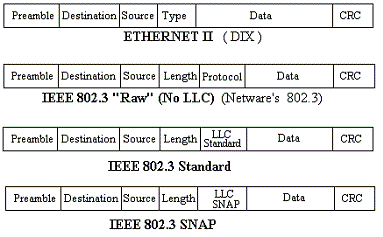
\includegraphics[width=0.6\textwidth]{media/tramas-ethernet.png}
\end{center}

\subsection{\href{https://es.wikipedia.org/wiki/IEEE\_802.2}{LLC}}
\label{sec:org4c7fa1c}
\begin{center}
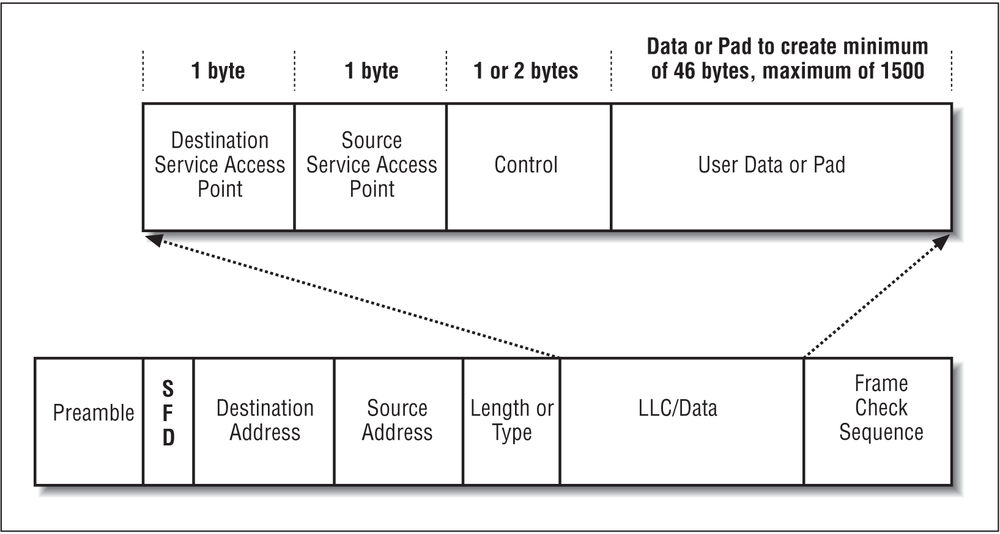
\includegraphics[width=0.6\textwidth]{media/llc.png}
\end{center}
\begin{itemize}
\item \textbf{DSAP} y \textbf{SSAP}: Especifican los protocolos de nivel superior
\item Control:
\begin{itemize}
\item Paquetes \textbf{U} , con un campo de control de 8 bits, están pensados para servicios no orientados a conexión. Son los usados \emph{normalmente}
\item Paquetes \textbf{I}, con un campo de control y secuencia numérica de 16 bits, están pensados para servicios orientados a conexión
\item Paquetes \textbf{S}, con un campo de control de 16 bits, están pensados para usarse en funciones supervisoras en la capa LLC (Logical Link Control).
\end{itemize}
\end{itemize}

\begin{NOTES}
\begin{itemize}
\item Lista de dsap-ssap:
\begin{itemize}
\item \url{http://standards.ieee.org/develop/regauth/llc/public.html}
\end{itemize}
\end{itemize}
\end{NOTES}
\subsection{\href{https://en.wikipedia.org/wiki/Subnetwork\_Access\_Protocol}{SNAP}}
\label{sec:orgb26d9f1}
\begin{itemize}
\item Cuando DSAP y SSAP tienen el valor \texttt{0xAA}
\item Distingue protocolos adicionales a los de LLC
\begin{itemize}
\item Por ejemplo, no hay un número asignado para que IP viaje sobre LLC
\end{itemize}
\end{itemize}

\subsection{¿Se usa LLC, SNAP?}
\label{sec:org0d7bf1b}
\emph{As per IETF RFC 1042, IP datagrams and ARP datagrams are transmitted over IEEE 802 networks using LLC and SNAP headers, except on Ethernet/IEEE 802.3, where they are transmitted with Ethernet II headers, as per RFC 894}
\begin{itemize}
\item Lo normal son tramas Ethernet-DIX, o 802.3 Raw
\end{itemize}


\subsection{Tamaño}
\label{sec:org5f45bd7}
\begin{itemize}
\item Tamaño mínimo: 64 bytes (46 de datos)
\begin{itemize}
\item Se necesita un \textbf{mínimo} para poder detectar las colisiones en \href{https://es.wikipedia.org/wiki/10BASE-T}{10baseT} (2500 metros máximos a 10Mbs)
\end{itemize}
\item Tamaño máximo: 1518 bytes (1500 de datos)
\begin{itemize}
\item Para limitar las colisiones y mejorar la compartición del medio
\end{itemize}
\item Estos límites son \textbf{obsoletos}
\begin{itemize}
\item Con los switches no hay colisiones
\item Mayores velocidades permiten \href{https://en.wikipedia.org/wiki/Jumbo\_frame}{tramas jumbo}
\end{itemize}
\end{itemize}

\subsubsection{MTU}
\label{sec:orgbcb19cc}
\begin{itemize}
\item \emph{Maximum Transfer Unit}
\item El sistema operativo puede permitir configurarlo para 
\begin{itemize}
\item Mejorar el rendimiento: tramas jumbo
\item Reducir la latencia: tramas más pequeñas
\end{itemize}

\begin{longtable}{lr}
\caption{MTU por defecto para algunas redes}
\\
Network & MTU (bytes)\\
\hline
\endfirsthead
\multicolumn{2}{l}{Continúa de la página anterior} \\
\hline

Network & MTU (bytes) \\

\hline
\endhead
\hline\multicolumn{2}{r}{Continúa en la siguiente página} \\
\endfoot
\endlastfoot
\hline
16 Mbps Token Ring & 17914\\
4 Mbps Token Ring & 4464\\
FDDI & 4352\\
Ethernet & 1500\\
IEEE 802.3/802.2 & 1492\\
PPPoE (WAN Miniport) & 1480\\
X.25 & 576\\
\end{longtable}
\end{itemize}


\section{Direcciones MAC}
\label{sec:org508253b}
\begin{itemize}
\item Se llaman \textbf{direcciones físicas}, aunque son de la capa de enlace
\item Son números de 48 bits (6 bytes). 
\begin{itemize}
\item Se expresan como números hexadecimales separados por dos puntos (\texttt{D4:AA:12:F3:00:C8})
\item En ocasiones (Windows) se utiliza como separador un - (\texttt{D4-AA-12-F3-00-C8})
\end{itemize}
\item Cada tarjeta de red tiene una dirección MAC única
\begin{itemize}
\item 24 bits indican el fabricante
\item 24 bits como identificador de la tarjeta dentro del fabricante
\end{itemize}

\item Es posible consultar el fabricante de tu tarjeta de red desde la MAC en muchos sitios de la web
\begin{itemize}
\item \href{http://www.seguridadwireless.net/php/direccion-mac.php}{http://www.seguridadwireless.net/php/direccion-mac.php}
\item \href{http://standards-oui.ieee.org/oui/oui.txt}{http://standards-oui.ieee.org/oui/oui.txt}
\end{itemize}
\end{itemize}

\begin{NOTES}


\#!/bin/bash
\#\url{https://www.linux.com/blog/handy-2-line-script-lookup-network-card-manufacturer-mac-address}
OUI=\$(echo \$\{1//[:.- ]/\} | tr "[a-f]" "[A-F]" | egrep -o "\^{}[0-9A-F]\{6\}")
grep \$OUI lynx -dump \url{http://standards.ieee.org/regauth/oui/oui.txt}
\end{NOTES}

\subsection{Consultar la propia MAC}
\label{sec:orgad6b110}
\begin{itemize}
\item Windows
\texttt{ipconfig /all}
\item Linux
\texttt{ifconfig -a | grep HWaddr}
\end{itemize}
La dirección MAC: FF:FF:FF:FF:FF:FF es de broadcast, e implica que los destinatarios del paquete enviado son todos los equipos de la subred.

\subsection{¿Puedo cambiar mi MAC?}
\label{sec:orgf7d3a9b}
\begin{itemize}
\item El sistema operativo consulta la MAC de la tarjeta
\item Después, la usa para enviar tramas
\item Pero se puede utilizar otra MAC a voluntad
\begin{itemize}
\item Máquinas virtuales
\item Con comandos/utilidades del sistema operativo
\end{itemize}
\end{itemize}

\lstset{language=shell,label= ,caption= ,captionpos=b,numbers=none}
\begin{lstlisting}
ifconfig eth0 down
ifconfig eth0 hw ether 60:6c:66:b5:85:65
ifconfig eth0 up
\end{lstlisting}



Protocolo ARP Es un protocolo que se encuentra en la frontera de las capas de red y enlace, aunque generalmente aparece como protocolo de red.  Permite determinar la dirección MAC de un equipo de nuestra misma subred conocida su dirección IP, para hacer la entrega de la trama localmente. Esta tarea la realiza el sistema operativo de nuestra máquina de forma transparente al usuario.  Cada vez que se hace una consulta para determinar la dirección física, el sistema operativo almacena temporalmente en una tabla la correspondencia de las direcciones IP y MAC para evitar repetir el proceso en futuros envíos.


Protocolo ARP Desde una sesión de consola, podemos consultar la información actual de la tabla ARP con el comando: arp –a.  Otros parámetros aceptados por el comando arp son:
\begin{itemize}
\item arp –d. Borra entradas en la tabla arp.
\item arp –s. Permite introducir entradas estáticas en la tabla arp.
\item Consulta el resto de opciones disponibles introduciendo el comando
\end{itemize}
arp sin parámetros.


Otros estándares 802.5 Token ring: utiliza el algoritmo de paso de testigo para regular el acceso al medio.  El testigo pasa de ordenador a ordenador (conectados en anillo) y si un ordenador quiere transmitir, puede hacerlo (por un tiempo limitado) cuando posee el testigo Usa codificación Manchester diferencial Existen especificaciones para lograr 1Gbps.  802.4 Token bus: es una mezcla entre ethernet y token ring. Se utiliza el paso de testigo en una red que tiene topología bus







\section{Referencias}
\label{sec:orgbda1485}
\begin{itemize}
\item Formatos:
\begin{itemize}
\item \href{par-03-capa-de-enlace.html}{Transparencias}
\item \href{par-03-capa-de-enlace.pdf}{PDF}
\end{itemize}
\item Creado con:
\begin{itemize}
\item \href{https://www.gnu.org/s/emacs/}{Emacs}
\item \href{https://github.com/yjwen/org-reveal}{org-reveal}
\item \href{https://www.latex-project.org/}{Latex}
\end{itemize}
\end{itemize}
\end{document}